%! suppress = FigureNotReferenced
%! suppress = Unicode
\documentclass{classrep}
\usepackage[utf8]{inputenc}
\usepackage{color}
\usepackage{graphicx}
\usepackage{hyperref}

\DeclareUnicodeCharacter{00A0}{~}

\studycycle{Informatyka, studia dzienne, inż I st.}
\coursesemester{IV}

\coursename{Sztuczna inteligencja i systemy ekspertowe}
\courseyear{2024/2025}

\courseteacher{dr inż. Krzysztof Lichy}
\coursegroup{Wtorek, 12:15}

\author{
    \studentinfo{Aleksander Gencel}{251517} \and
    \studentinfo{Bartosz Żelaziński}{251670}
}

\title{Zadanie 1: Piętnastka}

\begin{document}
    \maketitle
    \tableofcontents
    \clearpage


    \section{Cel}\label{sec:cel}
    Celem zadanie było zapoznanie się z algorytmami przechodzenia (bądź też przeszukiwania) grafów.
    Takimi są bowiem algorytmy Deep-First Search (DFS) oraz Breadth-First Search (BFS).
    Ten pierwszy to algorytm przeszukiwania grafu w głąb, natomiast ten drugi przeszukuje graf wszerz.


    \section{Wprowadzenie}\label{sec:wprowadzenie}
    Piętnastka to gra, która polega na rozwiązaniu układanki w taki sposób, żeby spośród rozsypanych liczb przesunąć
    cyfrę 0 tak, aby cała gra była ułożona po kolei z zerem na końcu.
    Aby rozwiązać przykładową grę w tabeli~\ref{tab:fifteen-example} należy zwyczajnie wykonać dwa ruchy w dół.

    \begin{table}[!h]
        \centering
        \begin{tabular}{|c|c|c|c|c|c|c|c|c|}
            \cline{1-4}\cline{6-9}
            1  & 2  & 3  & \textbf{0} & & 1  & 2  & 3  & 4          \\
            \cline{1-4}\cline{6-9}
            5  & 6  & 7  & 4          & & 5  & 6  & 7  & 8          \\
            \cline{1-4}\cline{6-9}
            9  & 10 & 11 & 8          & & 9  & 10 & 11 & 12         \\
            \cline{1-4}\cline{6-9}
            13 & 14 & 15 & 12         & & 13 & 14 & 15 & \textbf{0} \\
            \cline{1-4}\cline{6-9}
        \end{tabular}
        \caption{Gra w piętnastkę. Gra początkowa po lewej, gra rozwiązana po prawej. \cite{freelancinggig}}
        \label{tab:fifteen-example}
    \end{table}

    Zaprezentowane poniżej algorytmy mogą być wykorzystywane nie tylko do rozwiązywania problemu piętnastki,
    ale także do rozwiązywania innych problemów, które można przedstawić w postaci grafu.
    Każdy z nich ma swoje charakterystyczne cechy, różnią się między innymi wydajnością.

    \subsection{Algorytm BFS}\label{subsec:algorytm-bfs}
    Algorytm przeszukiwania wszerz (ang. \textit{Breadth-First Search}, BFS) jest algorytmem przeszukiwania grafu,
    który gwarantuje na znalezienie najkrótszej ścieżki w grafie.
    Wykorzystuje on w implementacji kolejkę FIFO, co pozwala na przeszukiwanie grafu poziomami.
    Charakteryzuje go przede wszystkim szybkość działania i nieduże zużycie pamięci. \cite{kielce}

    \begin{figure}[h]
        \centering
        
\includegraphics[width=0.5\linewidth]{src/bfs}
        \caption{Kolejność przeszukiwania drzewa w algorytmie BFS. \cite{wikibfs}}
        \label{fig:bfs}
    \end{figure}

    \subsection{Algorytm DFS}\label{subsec:algorytm-dfs}
    Algorytm ten przeszukuje graf w sposób charakterystyczny -- poprzez zagłębianie się w głąb struktury grafu aż do
    osiągnięcia zadanej maksymalnej głębokości lub do momentu, w którym znajdzie rozwiązanie.
    Stąd wywodzi się jego nazwa algorytmu przeszukiwania w głąb (ang. \textit{Deep-First Search}, DFS).
    W przeciwieństwie do algorytmu BFS korzysta on ze stosu LIFO i w tej implementacji jest wolniejszy. \cite{kielce}

    \begin{figure}[h]
        \centering
        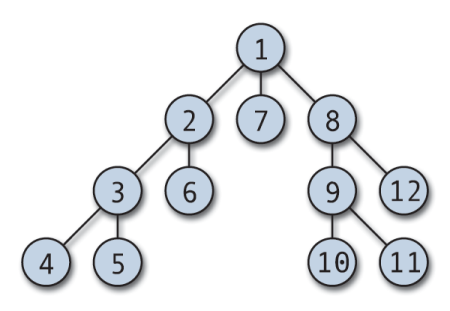
\includegraphics[width=0.5\linewidth]{src/dfs}
        \caption{Kolejność przeszukiwania drzewa w algorytmie DFS. \cite{wikidfs}}
        \label{fig:dfs}
        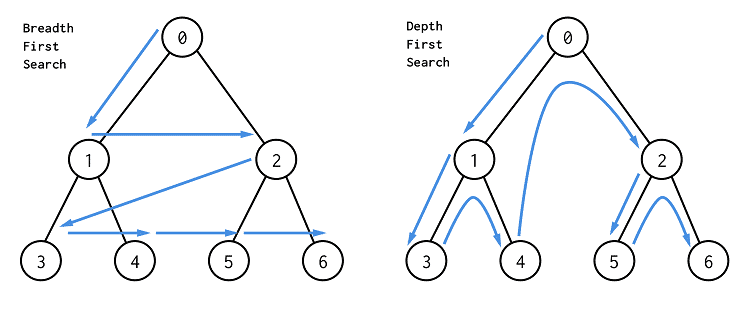
\includegraphics[width=\linewidth]{src/bfs-vs-dfs}
        \caption{Porównanie sposobu przeszukiwania algorytmów BFS (lewo) i DFS (prawo).}
        \label{fig:bfs-vs-dfs}
    \end{figure}

    \subsection{Algorytm A-star (A*)}\label{subsec:algorytm-a-star}
    Ten algorytm jest algorytmem heurystycznym.
    Posługując się funkcją
    \begin{equation}
        f(x) = g(x) + h(x),\label{eq:a-star-fx}
    \end{equation}
    gdzie $g(x)$ to koszt dotarcia do węzła $x$, a $h(x)$ to koszt dotarcia z węzła $x$ do celu, algorytm A-star
    przeszukuje te wierzchołki, które mają najmniejszą wartość tej funkcji. \cite{jarabas}
    Wybrano dwie heurystyki:
    \begin{enumerate}
        \item metryka Hamminga -- wartość obliczana na podstawie liczby elementów, które nie są na swoim miejscu,
        \item metryka Manhattan -- wartość obliczana na podstawie sumy odległości w poziomie i pionie.
    \end{enumerate}


    \section{Opis implementacji}\label{sec:opis-implementacji}
    To sprawozdanie dotyczy wersji 1.0 programu.
    Algorytmy BFS, DFS oraz A-star zostały zaimplementowane w Javie w wersji 8, choć początkowo były pisane w wersji 21.
    Jest to bardzo prosta aplikacja konsolowa, uruchamiana poleceniem
    \begin{center}
        \texttt{java -jar ./target/fifteen-game-1.0.jar <algorytm> <strategia> <plik\_gry> [plik\_rozw] [plik\_stat]},
    \end{center}
    co jest zgodne z przykładowymi wywołaniami opisanymi w instrukcji.
    Wykorzystywane są również skrypty do weryfikacji poprawności rozwiązań otrzymanych przez każdy algorytm oraz programy,
    które zostały udostępnione przez autora ćwiczenia.
    Każde wykonanie algorytmu zapisuje statystyki jego działania w obiekcie \textt{GameStat}.
    Gra przechowuje wysokość i szerokość układanki oraz jednowymiarową listę szesnastu liczb rzeczywistych,
    odpowiadającej ułożeniu liczb.
    Implementacje algorytmów w tym programie nie należą do najbardziej zaawansowanych, natomiast w zdecydowanej
    większości przypadków działają poprawnie.

    Diagram programu został przedstawiony na rysunku~\ref{fig:fifteen-diagram}.

    \subsection{Implementacja BFS}\label{subsec:implementacja-bfs}
    Algorytm BFS został zaimplementowany w klasie \texttt{FifteenBFSSolver.java}.
    Wykorzystuje on kolejkę (Queue), która jest kolekcją FIFO -- First In First Out.

    \subsection{Implementacja DFS}\label{subsec:implementacja-dfs}
    Algorytm DFS został zaimplementowany w klasie \texttt{FifteenDFSSolver.java}.
    Wykorzystuje on stos (Stack), który jest kolekcją LIFO -- Last In First Out.
    Pozwala to zatem na cofanie się oraz założono na stałe maksymalną głębokość schodzenia algorytmu do 20.

    \subsection{Implementacja A-star}\label{subsec:implementacja-a-star}
    Algorytm A-star został zaimplementowany w klasie \texttt{FifteenAStarSolver.java}.
    Wykorzystuje ona kolejkę priorytetową (PriorityQueue), która, jak opisano w rozdziale~\ref{subsec:algorytm-a-star},
    korzysta z funkcji~\ref{eq:a-star-fx} by obliczyć do pobrania kolejnego stanu o najmniejszej jej wartości.

    \clearpage

    \begin{figure}[!h]
        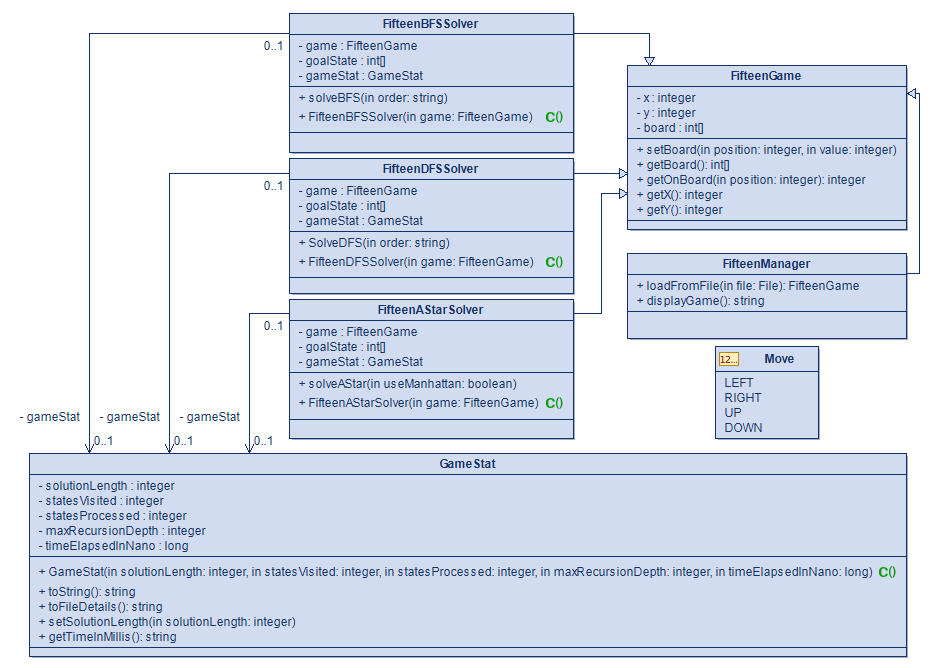
\includegraphics[width=\linewidth]{src/fifteen-diagram}
        \caption{Diagram programu.}
        \label{fig:fifteen-diagram}
    \end{figure}


    \section{Materiały i metody}\label{sec:materiay-i-metody}
    Metodą sprawdzania poprawności algorytmów do pewnego stopnia zaawansowania gry było rozpisanie tych gier ręcznie,
    w celu weryfikacji rozwiązań, gdyż nie są one zbytnio skomplikowane.
    Zgodnie z instrukcją, przy pomocy załączonych programów, tj. \texttt{puzzlegen.jar} wygenerowano gry o rozmiarze
    4 × 4 i głębokości 7.
    Następnie wykorzystano program \texttt{fifteen-game-1.0.jar} do rozwiązania tych gier, a potem \texttt{puzzleval.jar}
    do sprawdzenia ich poprawności.
    Proces cały zautomatyzowano, wykorzystując kolejno skrypty: \texttt{runprog.sh} oraz \texttt{runval.sh}.
    Do przeprowadzenia analizy, użyto skryptu \texttt{extdata.sh}, który podsumował wszystkie wyniki z wygenerowanych
    plików przez algorytmy.
    W języku python wykonano wykresy, które zostaną omówione w rozdziale~\ref{sec:wyniki}.

    \clearpage


    \section{Wyniki}\label{sec:wyniki}
    W tej sekcji, dla każdego algorytmu (astr, bfs, dfs) przedstawione zostaną wykresy przedstawiające:
    \begin{itemize}
        \item długość znalezionego rozwiązania,
        \item liczbę stanów odwiedzonych,
        \item liczbę stanów przetworzonych,
        \item maksymalną osiągniętą głębokość rekursji,
        \item czas trwania procesu obliczeniowego.
    \end{itemize}

    Dodatkowo ze skryptu \textt{runval.sh} wiemy, że:
    \begin{center}
        \texttt{
            \begin{tabular}{l}
                ----- Summary -----     \\
                Correct solutions: 6436 \\
                Incorrect solutions: 998
            \end{tabular}
        }
    \end{center}

    co oznacza, że 13,4\% rozwiązań było niepoprawnych.
    Wszystkie niepoprawne wyniki należały do DFS, który zwyczajnie ich nie znalazł, tj.\ zapisane zostało -1.

    \subsection{BFS (bfs)}\label{subsec:bfs-(bfs)}

    \begin{figure}[!h]
        \centering
        \includegraphics[width=\linewidth]{../plots/długość_bfs_vs_porządki}
        \caption{Długość znalezionego rozwiązania w algorytmie BFS.}
        \label{fig:bfs-dlugosc}
    \end{figure}

    \begin{figure}[!h]
        \centering
        \includegraphics[width=\linewidth]{../plots/odwiedzone_bfs_vs_porządki}
        \caption{Odwiedzone stany w algorytmie BFS.}
        \label{fig:bfs-odwiedzone}
        \includegraphics[width=\linewidth]{../plots/przetworzone_bfs_vs_porządki}
        \caption{Przetworzone stany w algorytmie BFS.}
        \label{fig:bfs-przetworzone}
    \end{figure}

    \begin{figure}[!h]
        \centering
        \includegraphics[width=\linewidth]{../plots/maks_głębokość_bfs_vs_porządki}
        \caption{Maksymalna osiągnięta głębokość rekursji w algorytmie BFS.}
        \label{fig:bfs-max-depth}
        \includegraphics[width=\linewidth]{../plots/czas_bfs_vs_porządki}
        \caption{Czas trwania procesu obliczeniowego w algorytmie BFS.}
        \label{fig:bfs-czas}
    \end{figure}

    \clearpage

    \subsection{DFS (dfs)}\label{subsec:dfs-(dfs)}

    \begin{figure}[!h]
        \centering
        \includegraphics[width=\linewidth]{../plots/długość_dfs_vs_porządki}
        \caption{Długość znalezionego rozwiązania w algorytmie DFS.}
        \label{fig:dfs-dlugosc}
        \includegraphics[width=\linewidth]{../plots/odwiedzone_dfs_vs_porządki}
        \caption{Odwiedzone stany w algorytmie DFS.}
        \label{fig:dfs-odwiedzone}
    \end{figure}

    \begin{figure}[!h]
        \centering
        \includegraphics[width=\linewidth]{../plots/przetworzone_dfs_vs_porządki}
        \caption{Przetworzone stany w algorytmie DFS.}
        \label{fig:dfs-przetworzone}
        \includegraphics[width=\linewidth]{../plots/maks_głębokość_dfs_vs_porządki}
        \caption{Maksymalna osiągnięta głębokość rekursji w algorytmie DFS.}
        \label{fig:dfs-max-depth}
    \end{figure}

    \begin{figure}[!h]
        \centering
        \includegraphics[width=\linewidth]{../plots/czas_dfs_vs_porządki}
        \caption{Czas trwania procesu obliczeniowego w algorytmie DFS.}
        \label{fig:dfs-czas}
    \end{figure}

    \clearpage

    \subsection{A-star (astr)}\label{subsec:a-star-(astr)}
    \begin{figure}[!h]
        \centering
        \includegraphics[width=\linewidth]{../plots/długość_astar_vs_heurystyka}
        \caption{Długość znalezionego rozwiązania w algorytmie A-star.}
        \label{fig:astar-dlugosc}
        \includegraphics[width=\linewidth]{../plots/odwiedzone_astar_vs_heurystyka}
        \caption{Odwiedzone stany w algorytmie A-star.}
        \label{fig:astar-odwiedzone}
    \end{figure}

    \begin{figure}[!h]
        \centering
        \includegraphics[width=\linewidth]{../plots/przetworzone_astar_vs_heurystyka}
        \caption{Przetworzone stany w algorytmie A-star.}
        \label{fig:astar-przetworzone}
        \includegraphics[width=\linewidth]{../plots/maks_głębokość_astar_vs_heurystyka}
        \caption{Maksymalna osiągnięta głębokość rekursji w algorytmie A-star.}
        \label{fig:astar-max-depth}
    \end{figure}

    \begin{figure}[!h]
        \centering
        \includegraphics[width=\linewidth]{../plots/czas_astar_vs_heurystyka}
        \caption{Czas trwania procesu obliczeniowego w algorytmie A-star.}
        \label{fig:astar-czas}
    \end{figure}

    \clearpage


    \section{Dyskusja}\label{sec:dyskusja}

    \subsection{BFS}\label{subsec:bfs}
    Jeden z szybszych algorytmów, który za każdym razem podał wynik.
    Widać, że długości rozwiązań są takie same jak głębokość gry.
    Zauważa się pewny błąd w przypadku czasu trwania algorytmu BFS w kolejności RDUL, co widać na rysunku~\ref{fig:bfs-czas}.
    Wartość ta jest najwyższa z możliwych, bo aż dwie i pół sekundy i nie była ona przewidywana.

    \subsection{DFS}\label{subsec:dfs}
    Zdecydowanie najgorszy algorytm do rozwiązywania piętnastki.
    Prawdopodobnie wynika to z błędnej, a raczej nieoptymalnej implementacji, gdyż algorytm często zapętla lub ostatecznie
    nawet nie znajduje rozwiązania.
    Zauważa się również, że temu algorytmowi najdłużej zajmuje znalezienie jakiegokolwiek rozwiązania.
    Nie ma również pewności, iż takowe zostanie odnalezione, a jeśli nawet, to niekoniecznie będzie ono optymalne bądź poprawne.

    \subsection{A-star}\label{subsec:a-star}
    Od razu można zauważyć, że algorytm jest zdecydowanie najszybszy wśród pozostałych, choć przy odległości Manhattan widać
    problem podobny do BFS, gdzie czas działania algorytmu jest znacznie dłuższy od pozostałych, bo aż sześciokrotnie od średniej.
    Zauważono pewny błąd co do strategii Hamminga, gdzie algorytm często przegrywał w wydajności w porównaniu do strategii Manhattana.
    Szczególnie widać to na wykresie odwiedzonych stanów~\ref{fig:astar-odwiedzone}, gdzie są one sześciokrotnie większe
    niż w przypadku drugiej strategii przy głębokości równej 7.


    \section{Wnioski}\label{sec:wnioski}
    \begin{enumerate}
        \item Najszybszym algorytmem okazuje się algorytm A-star, w badanym przypadku, z heurystyką odległości Manhattana.
        \item Algorytm DFS spisał się najgorzej z całej trójki.
        Istnieją przypadki, gdzie nie znajduje on rozwiązania, a jeśli je odnajdzie, to nie jest ono optymalne.
        \item Algorytmy BFS i A-star zawsze znalazły rozwiązanie.
        \item Różnica odwiedzonych oraz przetworzonych stanów w algorytmie DFS kontra BFS czy A-star jest diametralna.
        \item Algorytm A-star z heurystyką Hamminga działał gorzej niż z heurystyką Manhattana.
        \item Java jest dobrym językiem do implementacji tych algorytmów.
    \end{enumerate}

    \clearpage

    % apa quotation standard
    \begin{thebibliography}{0}
        \bibitem{freelancinggig} Gupta, K. (2019, luty 6). What is the difference between BFS and DFS algorithms. FreelancingGig.
        \href{https://www.freelancinggig.com/blog/2019/02/06/what-is-the-difference-between-bfs-and-dfs-algorithms/}{https://freelancinggig.com/...}
        \bibitem{wikibfs} Przeszukiwanie wszerz. (2024, lipiec 15). Wikipedia, wolna encyklopedia. Dostęp 14:53, kwiecień 7, 2025,
        Dostępny w Internecie: \href{https://www.pl.wikipedia.org/w/index.php?title=Przeszukiwanie_wszerz&oldid=74276741}{https://pl.wikipedia.org/...}
        \bibitem{wikidfs} Przeszukiwanie w głąb. (2024, sierpień 21). Wikipedia, wolna encyklopedia. Dostęp 14:53, kwiecień 7, 2025,
        Dostępny w Internecie: \href{https://www.pl.wikipedia.org/w/index.php?title=Przeszukiwanie\_w\_g%C5%82%C4%85b&oldid=74583679}{https://pl.wikipedia.org/...}
        \bibitem{kielce} Chrobot, A. (2019, czerwiec 2). Podstawy Programowania 2 - Algorytmy dfs i bfs. \href{https://achilles.tu.kielce.pl/portal/Members/84df831b59534bdc88bef09b15e73c99/archive/semestr-ii-2018-2019/pdf/pp2/lecture/pp2_lecture_13.pdf}{https://achilles.tu.kielce.pl/...}
        \bibitem{jarabas} Raczyńska, J. Algorytm A*. \href{https://elektron.elka.pw.edu.pl/~jarabas/ALHE/notatki3.pdf}{https://elektron.elka.pw.edu.pl/...}
    \end{thebibliography}

\end{document}
